\newpage
\hypertarget{initialize vis}{}
\subsection{First steps}
\visHeader

\begin{itemize}

\item[$\blacktriangleright$] From your Eclipse workspace, open the \texttt{Dict\-ion\-ary.eap} file in Enterprise Architect (EA). The project browser should
closely resemble Fig.~\ref{ea:mocaTagged}. As you can see, the project is already populated with \texttt{MocaTree} and other built-in metamodels
in the \texttt{eMoflon Languages} working set.

\vspace{0.5cm}

\begin{figure}[htpb]
\begin{center}
  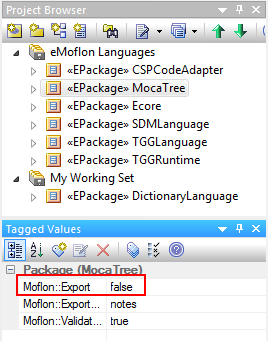
\includegraphics[width=0.4\textwidth]{ea_mocaTaggedValues}
  \caption{\texttt{MocaTree} is one of eMoflon's internal metamodels}
  \label{ea:mocaTagged}
\end{center}
\end{figure}

\end{itemize}

\vspace{-0.5cm}

If you inspect the tagged values\footnote{The ``Tagged Values'' window can be opened by going to ``View/Tagged Values'' or by hovering over the \texttt{Tagged
Values} tab immediately to the right of the project browser.} for these built-in languages, you'll notice that the \texttt{MocaTree} package has the
\texttt{Moflon::Export} value set to \texttt{false}. This ensures that the package is \emph{ignored} when exporting. As with all such standard metamodels (e.g.,
Ecore or our SDM metamodel) the \texttt{MocaTree} package in EA should be regarded as read-only, required in the EA project so that SDMs/TGGs can refer to
the classes defined in the package.

\begin{itemize}

\item[$\blacktriangleright$] Despite \texttt{DictionaryLanguage} being contained in a different working set than \texttt{MocaTree}, the two
metamodels are contained within the same EA project (EAP) which means you are able to create a new TGG using them both. Add a new package to \texttt{My
Working Set} named \texttt{Dict\-ion\-ary\-Code\-Adap\-ter}.

\item[$\blacktriangleright$] Select the package and add a new TGG schema diagram as depicted in Fig.~\ref{ea:newTGGDiagram}. In the next dialogue window,
set the source project as \texttt{MocaTree}, and the target project as \texttt{Dict\-ion\-ary\-Lang\-uage}.

\begin{figure}[h!]
\begin{center}
  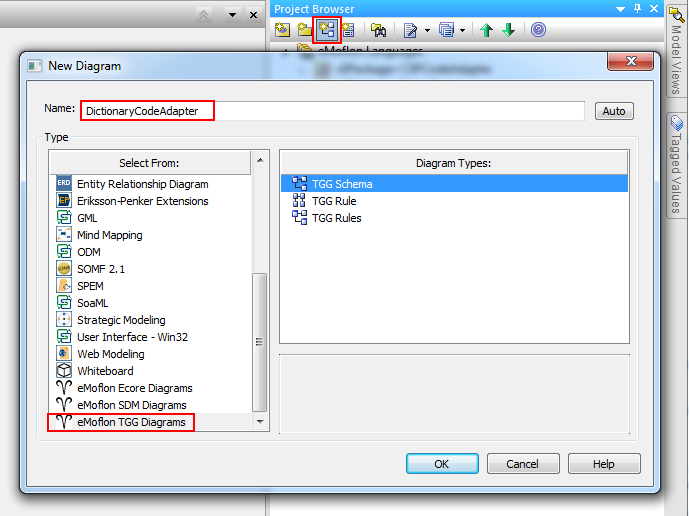
\includegraphics[width=0.9\textwidth]{ea_adapterTGGDiagram}
  \caption{Create a new TGG schema diagram}
  \label{ea:newTGGDiagram}
\end{center}
\end{figure}

\item[$\blacktriangleright$] For the moment, add a single correspondence type to the new diagram now active in the editor (the TGG \texttt{schema}) between
\texttt{Folder} and \texttt{Library}. Remember, you can get the classes by drag-and-dropping each element into the diagram, then quick-creating a new
\texttt{TGG~Cor\-res\-pon\-dence~Type} between them.\footnote{For details on the correspondence metamodel and how to create types, refer to Part IV, Section 3.}
Your diagram should come to resemble Fig.~\ref{ea:firstCorrType}.

\vspace{0.5cm}

\begin{figure}[htpb]
\begin{center}
  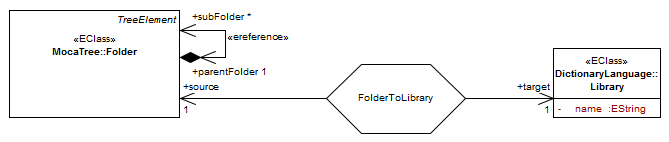
\includegraphics[width=\textwidth]{ea_firstAdapterCorrespondence}
  \caption{The first correspondence type for the transformation}
  \label{ea:firstCorrType}
\end{center}
\end{figure}

\newpage

\item[$\blacktriangleright$] Your complete project browser should now resemble Fig.~\ref{ea:TGGProjBrow}, where \texttt{Dict\-ion\-ary\-Code\-Adap\-ter} is now
explicitly listed as a \texttt{TGGSchemaPackage}.

\vspace{0.5cm}

\begin{figure}[htpb]
\begin{center}
  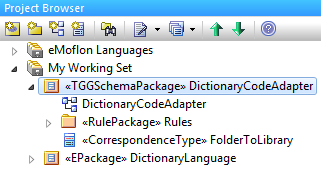
\includegraphics[width=0.5\textwidth]{ea_TGGProjectBrowser}
  \caption{A fully prepared TGG project}
  \label{ea:TGGProjBrow}
\end{center}
\end{figure}

\item[$\blacktriangleright$] Validate and export your file via the eMoflon control panel,\footnote{Activate via ``Extensions/Add-in Windows''} then switch
back to Eclipse and refresh the package explorer. A new \texttt{Dict\-ion\-ary\-Code\-Adap\-ter} project should appear in \texttt{My Working Set}.

\jumpSingle{subSec:setupParser}

\end{itemize}
